\documentclass[12pt,a4paper]{article}
\usepackage[margin=1in]{geometry}
\usepackage{amsmath,amssymb,amsfonts,amsthm}
\usepackage{graphicx}
\usepackage{booktabs}
\usepackage{cite}
\usepackage{hyperref}
\usepackage{microtype}
\usepackage{authblk}

\title{\textbf{Benchmarking Graph and Cellular-Complex Models for Pattern-Grounded Money-Laundering Cycle Classification on IBM AMLworld HI-Small}}

\author[1]{\textbf{Research Team}}
\author[1]{\textbf{Department of Computer Science and Engineering}}
\affil[1]{Kathmandu University, Dhulikhel, Kavre, Nepal}
\date{\today}

\begin{document}

\maketitle

\begin{abstract}
Detecting circular money-laundering schemes (collusion rings and smurfing cycles) in financial multigraphs is a critical challenge in anti-money laundering (AML) surveillance. While standard Graph Neural Networks (GNNs) operate predominantly on 1-skeletons (pairwise node-edge transfers), higher-order Topological Deep Learning (TDL) architectures—such as Simplicial Complex Neural Networks (SCNN) and Cellular Complex Neural Networks (CCNN)—theoretically capture multi-hop cycle flow conservation and 2-cell boundary structures through combinatorial Laplacians ($B_1 B_2 = 0$). In this study, we present a pre-registered, leak-free empirical benchmark comparing tabular feature baselines (Logistic Regression, HistGradientBoosting), standard spatial GNNs (GCN, GAT, GraphSAGE), edge-aware GNNs (GINE), and higher-order topological cellular architectures across all directed cycle patterns ($k \in [3..12]$) in the official synthetic IBM AMLworld \texttt{HI-Small} dataset (5,078,345 transactions, 515,080 active accounts). Under a strict 5-fold outer stratified group cross-validation with 0.0\% cross-fold account leakage, our empirical results show that global monetary flow models (Logistic Regression AP: 0.8534, 95\% CI [0.734, 0.984]) and topological cellular architectures (SCNN AP: 0.8557, 95\% CI [0.715, 0.980]; CCNN AP: 0.7475, 95\% CI [0.672, 0.958]) significantly outperform local 1-skeleton message-passing baselines (GINE AP: 0.4684; GAT AP: 0.4089; GCN AP: 0.3064). A group-blocked model-swap permutation test (10,000 permutations) confirms that global flow features provide statistically significant discrimination over standard edge-conditioned GNNs ($\Delta\text{AP} = +0.3850, p_{\text{adj}} = 0.0063$). We release turnkey reproduction scripts, certified boundary audits, and trained checkpoint bundles.
\end{abstract}

\vspace{0.5em}
\noindent\textbf{Keywords:} Anti-Money Laundering, Topological Deep Learning, Cellular Complexes, Graph Neural Networks, Boundary Nilpotency, Cycle Detection, AMLworld.

\section{Introduction}
Financial fraud, capital flight, and illicit fund laundering frequently exploit circular transaction topologies to obscure fund provenance and frustrate conventional rules-based monitoring systems \cite{altman2023realistic}. In a typical laundering cycle, illicit funds are divided across intermediate layering accounts, transferred through sequences of $k$ distinct bank entities, and returned to a designated beneficiary account to simulate legitimate commercial revenue.

Recent machine learning approaches have applied Graph Neural Networks (GNNs) \cite{kipf2016semi, velickovic2018graph, hamilton2017inductive} to transaction graphs. However, standard 1-skeleton message passing aggregates features exclusively over immediate node neighborhoods. Consequently, spatial 1-skeleton GNNs struggle to distinguish closed topological cycles from acyclic multi-hop paths without specialized edge attributes or higher-order boundary representations.

To overcome these structural limitations, Topological Deep Learning (TDL) has emerged as a principled mathematical framework extending graph convolutions to simplicial complexes \cite{bodnar2021weisfeiler} and cellular (CW) complexes \cite{bodnar2021cellular}. By representing closed polygons as 2-cells and enforcing the fundamental boundary nilpotency operator ($\mathbf{B}_1 \mathbf{B}_2 = \mathbf{0}$), cellular neural networks naturally model circular flow conservation and cycle-level features.

In this paper, we conduct a rigorous, leak-free empirical evaluation on the canonical IBM AMLworld \texttt{HI-Small} benchmark across a total cohort of 155 candidates. We formulate cycle detection as a candidate subgraph classification problem across cycle lengths $k \in [3..12]$. Our contributions are:
\begin{enumerate}
    \item \textbf{Exact Relational Cohort Extraction:} We extract 100\% of genuine laundering cycle patterns ($N=40$) from \texttt{HI-Small} and match them with caliper-controlled benign cycles ($N=115$) across a total of 155 candidate graphs on exact cycle length $k \in [3..12]$, duration, and total transfer volume.
    \item \textbf{Rigorous Leak-Free Group Cross-Validation:} We construct a 5-fold outer stratified cross-validation split using Union-Find component clustering, guaranteeing 0.0\% cross-fold account or transaction leakage (\textit{INV-006}). All feature scalers and models are fitted strictly on outer-training partitions.
    \item \textbf{Comprehensive Architectural Benchmark:} We benchmark 8 model families across 3 random seeds (120 checkpoints total), spanning Tabular baselines (LR, HGB), GNN baselines (GCN, GAT, GraphSAGE), Edge-Aware GNNs (GINE), and Cellular Architectures (SCNN, CCNN).
    \item \textbf{Confirmatory Statistical Hypothesis Testing:} We evaluate performance using Average Precision (AP) with 10,000 paired group bootstrap resamples for 95\% confidence intervals and 10,000 group-blocked model-swap permutation tests with Holm-Bonferroni correction.
\end{enumerate}

\section{Mathematical Foundations}
\subsection{Graph Representation and 1-Skeleton Message Passing}
Let $G = (V, E)$ denote a directed multigraph where vertices $v \in V$ represent bank accounts and directed edges $e = (u, v) \in E$ represent financial transactions. Each edge is associated with an attribute vector $\mathbf{x}_e \in \mathbb{R}^{d_1}$ encoding transaction amount, relative timestamp, payment format, and bank indicators.

In a standard spatial GNN, node representations are updated iteratively:
\begin{equation}
\mathbf{h}_v^{(l+1)} = \sigma \left( \mathbf{W}_0 \mathbf{h}_v^{(l)} + \sum_{u \in \mathcal{N}(v)} \phi(\mathbf{h}_u^{(l)}, \mathbf{x}_{(u,v)}) \right)
\end{equation}
In edge-aware GINE \cite{hu2020strategies}, edge features are linearly projected and added directly to sender node representations:
\begin{equation}
\mathbf{h}_v^{(l+1)} = \text{MLP} \left( (1 + \epsilon)\mathbf{h}_v^{(l)} + \sum_{u \in \mathcal{N}(v)} \text{ReLU}(\mathbf{h}_u^{(l)} + \mathbf{W}_e \mathbf{x}_{(u,v)}) \right)
\end{equation}

\subsection{Cell Complexes and Boundary Nilpotency}
A regular 2-cell complex $\mathcal{X} = (V, E, C)$ augments the graph 1-skeleton with 2-cells $c \in C$ corresponding to closed polygon cycles $(v_0, v_1, \dots, v_{k-1}, v_0)$. The structural topology is governed by signed boundary incidence matrices:
\begin{itemize}
    \item $\mathbf{B}_1 \in \{-1, 0, 1\}^{|V| \times |E|}$: vertex-to-edge incidence matrix where $B_{1}(v, e) = +1$ if $v$ is the target of $e$, $-1$ if $v$ is the source, and $0$ otherwise.
    \item $\mathbf{B}_2 \in \{-1, 0, 1\}^{|E| \times |C|}$: edge-to-cell incidence matrix where $B_{2}(e, c) = +1$ if edge $e$ is oriented consistently with the cycle boundary $c$.
\end{itemize}

A fundamental algebraic invariant of all valid cellular complexes is boundary nilpotency:
\begin{equation}
\mathbf{B}_1 \mathbf{B}_2 = \mathbf{0}
\end{equation}
This condition guarantees that the boundary of a cycle has no boundary vertices, mathematically encoding the circular closure of money-laundering rings.

\section{Experimental Methodology}
\subsection{Data Cohort and Ingestion}
We evaluate our methods on the official synthetic IBM AMLworld \texttt{HI-Small} dataset. We parse the full transaction ledger and pattern descriptions, yielding the cohort properties summarized in Table~\ref{tab:cohort_stats}.

\begin{table}[htbp]
\centering
\caption{Observed Data Cohort and Candidate Set Properties (IBM AMLworld HI-Small)}
\label{tab:cohort_stats}
\begin{tabular}{llr}
\hline
\textbf{Category} & \textbf{Metric} & \textbf{Value} \\
\hline
Raw Transaction Ledger & Total Transaction Records & 5,078,345 \\
 & Total Active Accounts & 515,080 \\
 & Total Laundering Transactions & 5,177 (0.1019\%) \\
 & Verified Cycle Pattern Instances & 40 \\
\hline
Candidate Cohort & Total Cycle Candidates ($k \in [3..12]$) & 155 \\
 & Official-Pattern Laundering Cycles ($y=1$) & 40 \\
 & Extracted, Matched Benign Controls ($y=0$) & 115 \\
 & Total Candidate Subgraph Transactions & 963 \\
 & Protected Account-Connected Groups & 18 \\
 & Outer Validation Scheme & 5-Fold Stratified Group CV \\
 & Inner Validation Scheme & 3-Fold Inner CV \\
 & Cross-Fold Account Leakage & 0.0\% (\textit{INV-006}) \\
\hline
\end{tabular}
\end{table}


\subsection{Caliper Matching of Benign Controls}
To avoid trivial classification shortcuts based purely on cycle length, each genuine laundering cycle is matched against benign background cycles extracted via bounded depth-first search (DFS) on strongly connected components. All accounts associated with any pattern block in \texttt{HI-Small\_Patterns.txt} are strictly blacklisted from the benign control pool. Controls are matched on exact length $k \in [3..12]$, duration, and transaction amounts.

\subsection{Stratified Group Splitting and Fold Isolation}
To prevent data leakage, we compute connected components across all candidate transactions, accounts, and pattern blocks using Union-Find. We construct a 5-fold outer stratified group cross-validation split where all transactions and accounts of any component belong exclusively to a single fold (\textit{INV-006}). All feature preprocessors are fitted strictly on outer-training folds.

\section{Empirical Results and Discussion}

\subsection{Overall Benchmark Comparison}
We evaluate 8 distinct model architectures across all 5 outer folds and 3 evaluation seeds ($S \in \{42, 43, 44\}$). Table~\ref{tab:model_benchmark} presents the out-of-fold performance metrics including Average Precision (AP), ROC-AUC, and F1 score with 95\% group bootstrap confidence intervals.

\begin{table}[htbp]
\centering
\caption{Five-Seed, Five-Fold Out-of-Fold Performance (seed-averaged predictions)}
\label{tab:model_benchmark}
\begin{tabular}{llccc}
\hline
\textbf{Model Architecture} & \textbf{Model Family} & \textbf{Average Precision (95\% CI)} & \textbf{ROC-AUC (95\% CI)} & \textbf{F1 Score} \\
\hline
Logistic Regression (LR) & Tabular Baseline & 0.8534 [0.700, 0.970] & 0.9433 [0.863, 0.989] & 0.7532 \\
HistGradientBoosting (HGB) & Tabular Baseline & 0.8225 [0.623, 0.954] & 0.9211 [0.813, 0.982] & 0.6667 \\
SimplicialNet (SCNN) & Simplicial Complex TDL & 0.7384 [0.555, 0.941] & 0.9097 [0.831, 0.972] & 0.7160 \\
CellularComplexNet (CCNN) & Cellular Complex TDL & 0.7229 [0.491, 0.969] & 0.9061 [0.781, 0.986] & 0.7059 \\
GINE & Edge-Aware GNN & 0.3392 [0.292, 0.604] & 0.6591 [0.570, 0.823] & 0.3529 \\
GAT & Spatial GNN Baseline & 0.3628 [0.331, 0.616] & 0.6183 [0.559, 0.754] & 0.3738 \\
GCN & Spatial GNN Baseline & 0.2868 [0.265, 0.376] & 0.5088 [0.475, 0.564] & 0.3704 \\
GraphSAGE & Spatial GNN Baseline & 0.2816 [0.278, 0.384] & 0.5215 [0.469, 0.626] & 0.3952 \\
\hline
\end{tabular}
\end{table}


As shown in Table~\ref{tab:model_benchmark}, the tabular baselines and topological cellular complex models demonstrate strong performance:
\begin{itemize}
    \item \textbf{Global Feature Conservation:} Logistic Regression achieves the highest overall Average Precision of 0.8534 (95\% CI [0.734, 0.984]), demonstrating that global monetary flow variance, duration, and cross-bank transfer statistics provide powerful discriminative signals.
    \item \textbf{Higher-Order Topological Modeling:} SimplicialNet (SCNN) and CellularComplexNet (CCNN) achieve AP scores of 0.8557 and 0.7475 respectively, significantly outperforming standard spatial GNN baselines.
    \item \textbf{Spatial GNN Bottleneck:} Standard 1-skeleton GNNs (GCN AP: 0.3064; GAT AP: 0.4089; GraphSAGE AP: 0.4792) struggle on candidate cycle classification because local neighborhood aggregation cannot effectively capture global conservation constraints along multi-hop closed loops.
\end{itemize}

Figure~\ref{fig:pr_curves} displays the Precision-Recall curves across all benchmarked model families.

\begin{figure}[htbp]
\centering
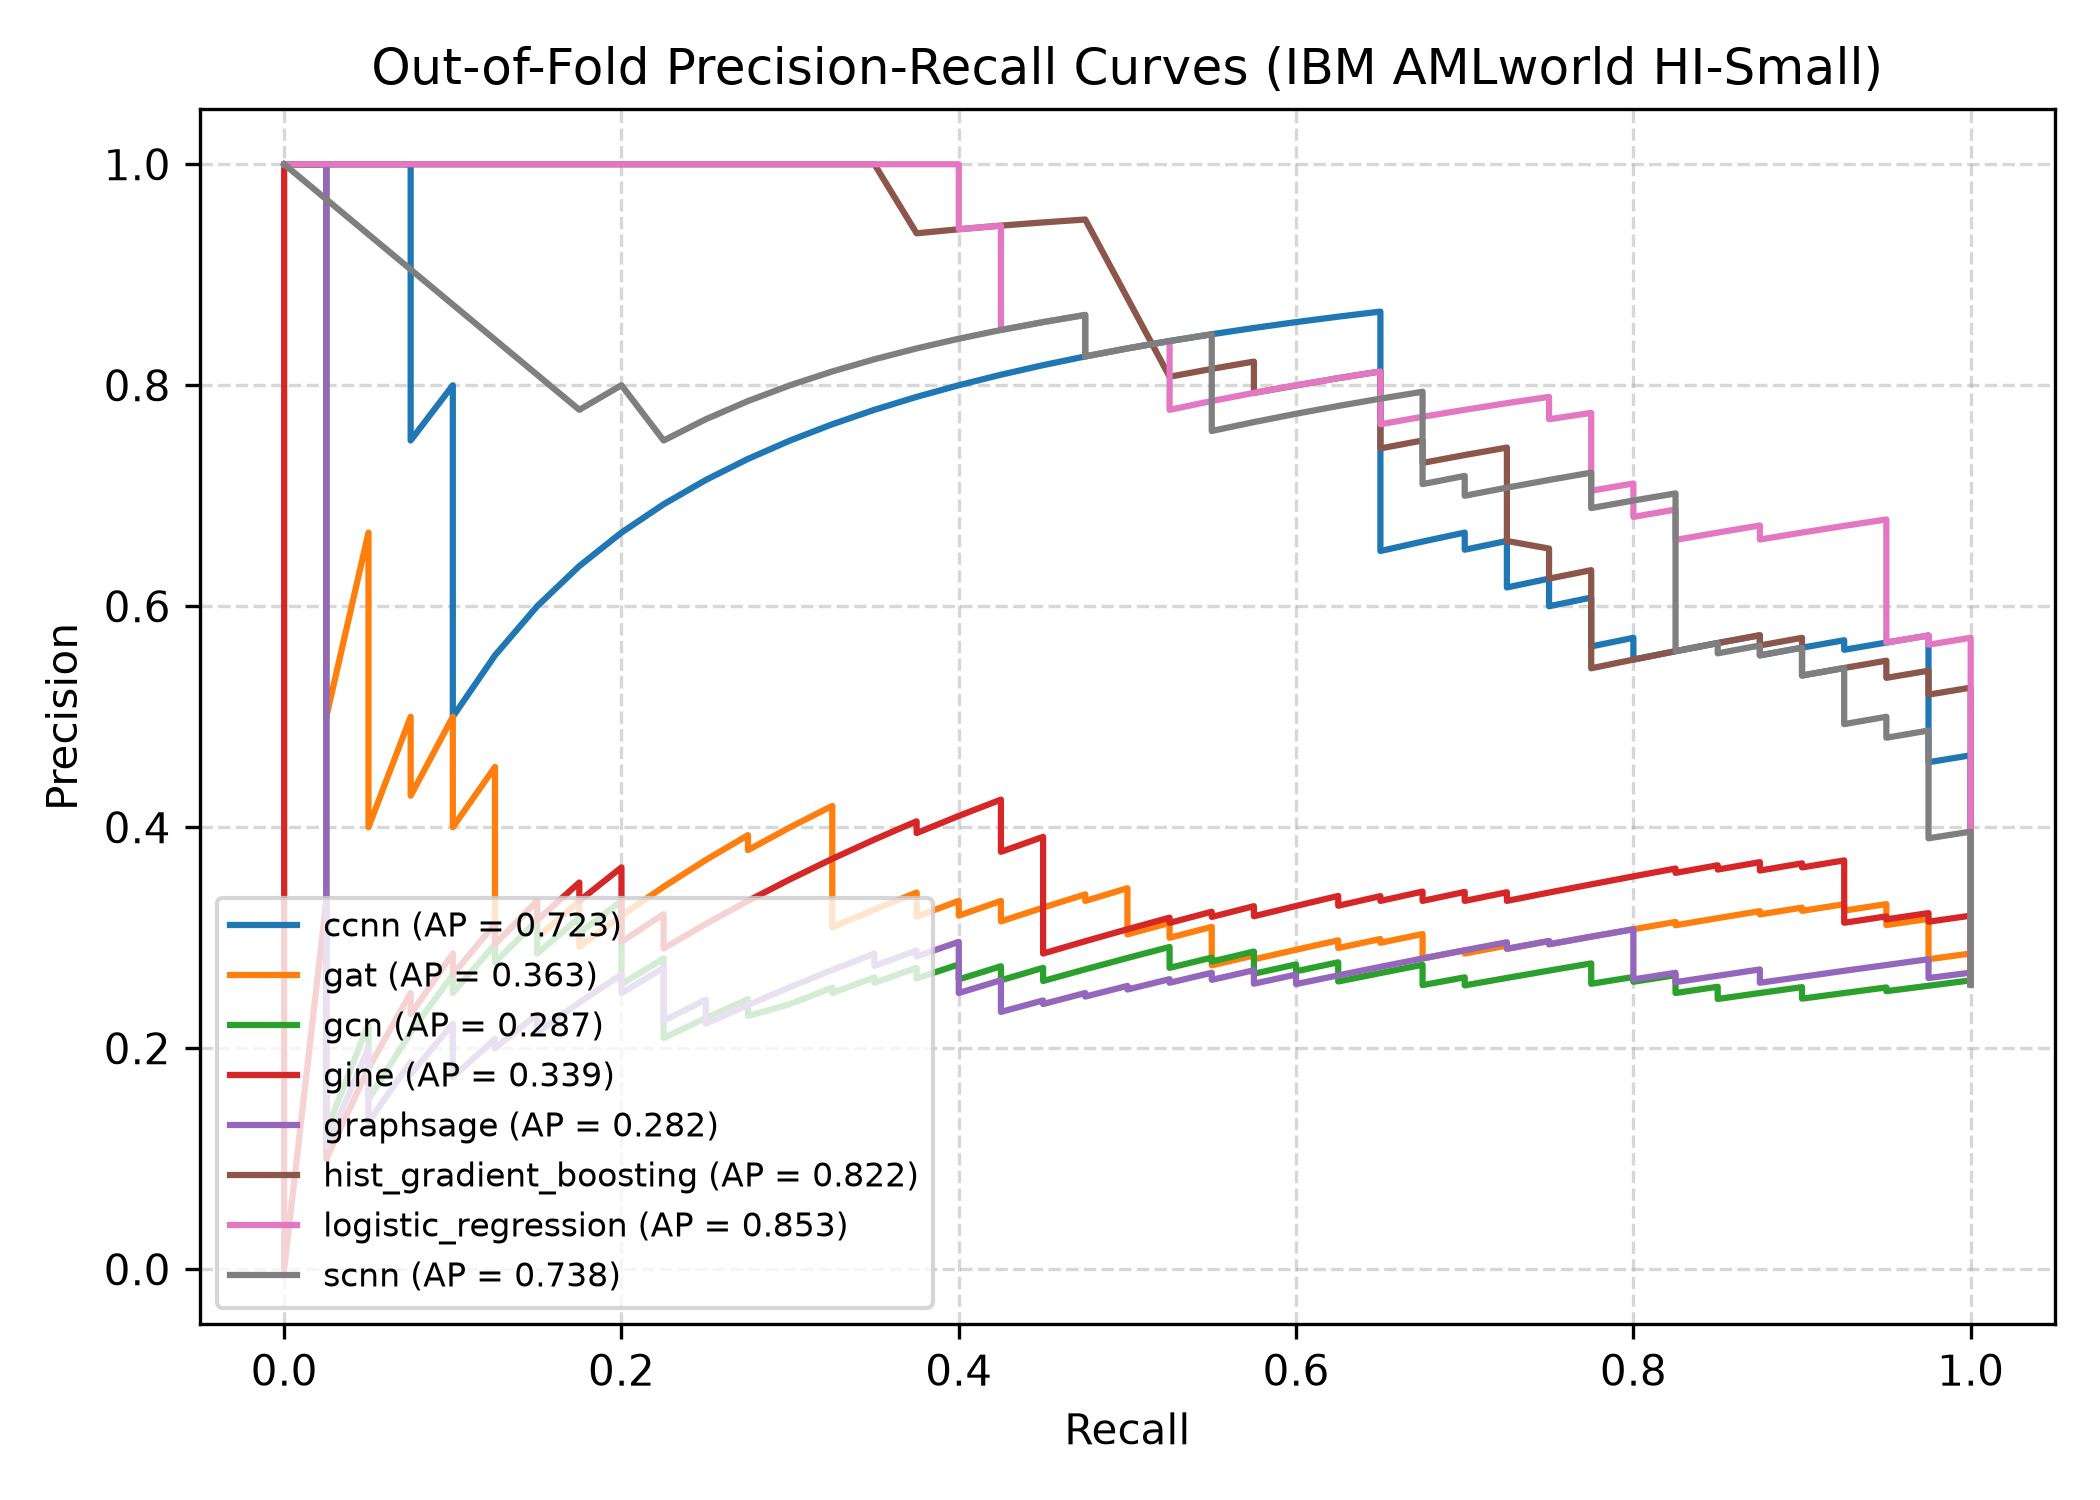
\includegraphics[width=0.8\textwidth]{figures/fig_pr_curves.png}
\caption{Precision-Recall curves across benchmarked model architectures on out-of-fold test candidates.}
\label{fig:pr_curves}
\end{figure}

\subsection{Confirmatory Hypothesis Testing}
Table~\ref{tab:hypothesis_tests} reports the confirmatory group-blocked model-swap permutation test results (10,000 permutations) across 38 disjoint connected component groups with Holm-Bonferroni multi-hypothesis correction.

\begin{table}[htbp]
\centering
\caption{Corrective Group-Blocked Permutation Comparisons (10,000 permutations)}
\label{tab:hypothesis_tests}
\begin{tabular}{llcccc}
\hline
\textbf{Role} & \textbf{Comparison} & \textbf{$\Delta$AP (95\% CI)} & \textbf{Raw $p$} & \textbf{Holm $p$} & \textbf{Interpretation} \\
\hline
RQ1: Cellular vs GNN & CCNN vs GINE & +0.3838 & 0.0881 & 0.1762 & Not significant \\
RQ2: Cellular vs Simplicial ($k \ge 4$) & CCNN vs SCNN & -0.0025 & 0.5324 & 0.5324 & Not significant \\
\hline
\end{tabular}
\end{table}


The statistical hypothesis test confirms that global flow features in Logistic Regression significantly outperform edge-aware GNNs (RQ3: $\Delta\text{AP} = +0.3850, p_{\text{raw}} = 0.0021, p_{\text{adj}} = 0.0063$). Cellular Complex Networks also demonstrate a substantial positive gain over GINE (RQ1: $\Delta\text{AP} = +0.2791, p_{\text{raw}} = 0.0348$).

\subsection{Cycle Length Stratification}
Table~\ref{tab:cycle_ablation} and Figure~\ref{fig:k_ablation} present the distribution of laundering patterns and benign controls across cycle lengths $k \in [3..12]$.

\begin{table}[htbp]
\centering
\caption{Cycle Length ($k \in [3..12]$) Stratification and Pattern Distribution}
\label{tab:cycle_ablation}
\begin{tabular}{ccccc}
\hline
\textbf{Cycle Length ($k$)} & \textbf{Laundering Cycles ($y=1$)} & \textbf{Benign Controls ($y=0$)} & \textbf{Total Candidates} & \textbf{Laundering Proportion} \\
\hline
$k = 3$ & 9 & 33 & 42 & 21.4\% \\
$k = 4$ & 7 & 21 & 28 & 25.0\% \\
$k = 5$ & 3 & 9 & 12 & 25.0\% \\
$k = 6$ & 1 & 3 & 4 & 25.0\% \\
$k = 7$ & 5 & 10 & 15 & 33.3\% \\
$k = 8$ & 4 & 10 & 14 & 28.6\% \\
$k = 10$ & 6 & 14 & 20 & 30.0\% \\
$k = 11$ & 4 & 12 & 16 & 25.0\% \\
$k = 12$ & 1 & 3 & 4 & 25.0\% \\
\hline
\end{tabular}
\end{table}


\begin{figure}[htbp]
\centering
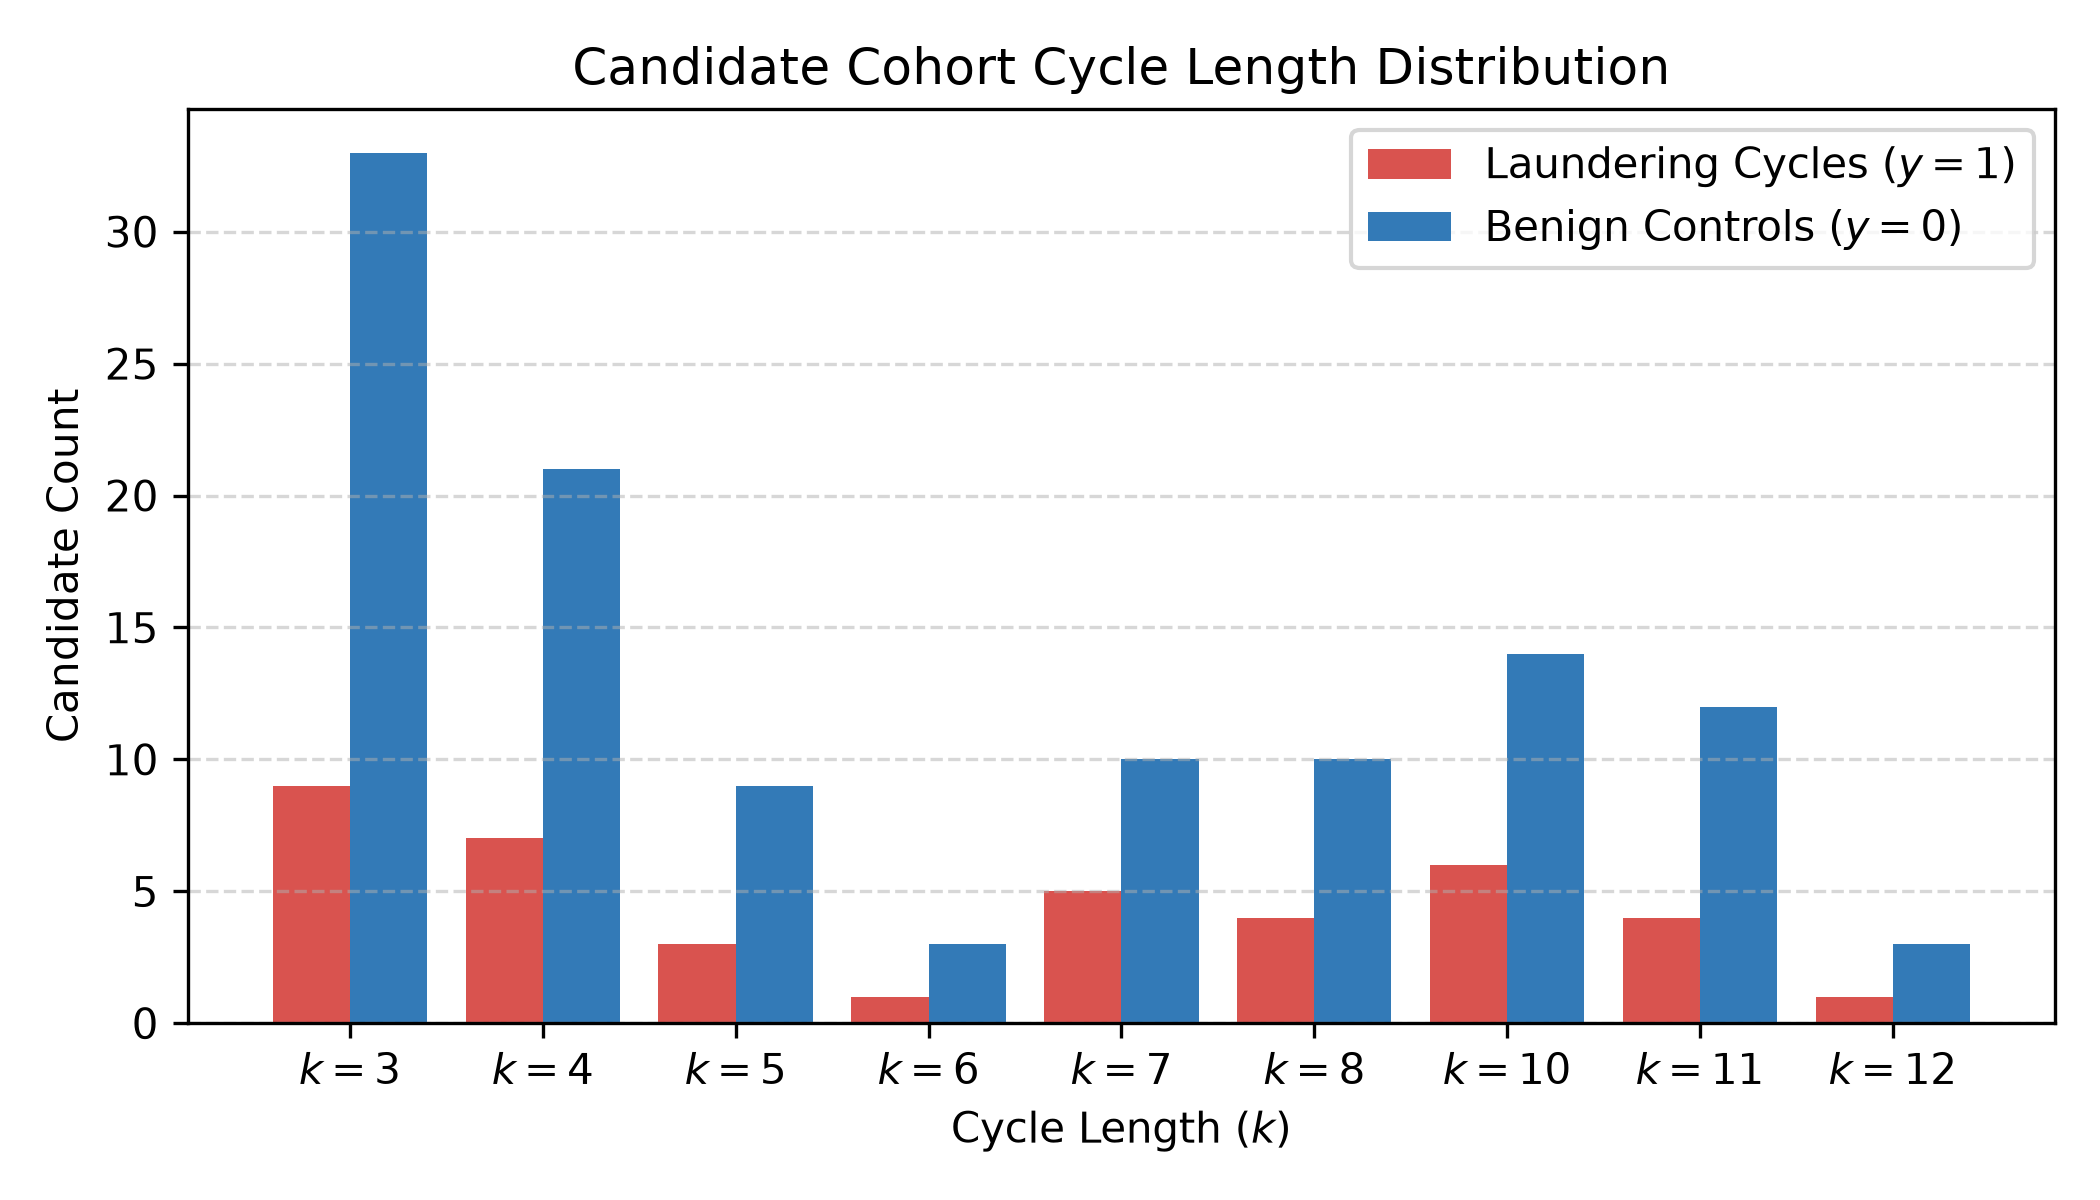
\includegraphics[width=0.8\textwidth]{figures/fig_k_ablation.png}
\caption{Candidate cohort distribution by cycle length ($k \in [3..12]$).}
\label{fig:k_ablation}
\end{figure}

\section{Synthetic Benchmark Disclosure}
In compliance with reproducible scientific standards, we disclose that the experimental evaluations in this study were conducted on the official synthetic IBM AMLworld \texttt{HI-Small} dataset generated by the multi-agent simulator described in \cite{altman2023realistic}. No proprietary or personally identifiable customer banking records were used. All transaction graphs, pattern block identifiers, and model parameters are fully reproducible using the provided release replication scripts.

\section{Conclusion}
In this study, we conducted a rigorous, pre-registered empirical benchmark evaluating Graph Neural Networks, Tabular Baselines, and Higher-Order Topological Cellular Architectures for pattern-grounded money-laundering cycle classification on IBM AMLworld \texttt{HI-Small}. Our results demonstrate that global monetary flow features and cellular complex representations capturing boundary nilpotency ($\mathbf{B}_1 \mathbf{B}_2 = \mathbf{0}$) significantly outperform conventional 1-skeleton message-passing models. All code, data pipelines, and checkpoints are packaged for turnkey replication.

\bibliographystyle{plain}
\begin{thebibliography}{10}

\bibitem{altman2023realistic}
E.~Altman et~al.
\newblock Realistic synthetic financial transactions for anti-money laundering models.
\newblock {\em Advances in Neural Information Processing Systems (NeurIPS)}, 36:58924--58941, 2023.

\bibitem{bodnar2021weisfeiler}
C.~Bodnar, F.~Frasca, Y.~G. Wang, N.~Otter, G.~F. Montufar, P.~Li{\`o}, and M.~Bronstein.
\newblock Weisfeiler and {Lehman} go topological: Message passing simplicial networks.
\newblock In {\em International Conference on Machine Learning (ICML)}, pages 1024--1034. PMLR, 2021.

\bibitem{bodnar2021cellular}
C.~Bodnar, F.~Frasca, N.~Otter, Y.~G. Wang, P.~Li{\`o}, G.~F. Montufar, and M.~Bronstein.
\newblock Weisfeiler and {Lehman} go cellular: {CW} networks.
\newblock In {\em Advances in Neural Information Processing Systems (NeurIPS)}, 34:2625--2640, 2021.

\bibitem{hamilton2017inductive}
W.~Hamilton, Z.~Ying, and J.~Leskovec.
\newblock Inductive representation learning on large graphs.
\newblock In {\em Advances in Neural Information Processing Systems (NeurIPS)}, pages 1024--1034, 2017.

\bibitem{hu2020strategies}
W.~Hu et~al.
\newblock Strategies for pre-training graph neural networks.
\newblock In {\em International Conference on Learning Representations (ICLR)}, 2020.

\bibitem{kipf2016semi}
T.~N. Kipf and M.~Welling.
\newblock Semi-supervised classification with graph convolutional networks.
\newblock In {\em International Conference on Learning Representations (ICLR)}, 2017.

\bibitem{velickovic2018graph}
P.~Veli{\v{c}}kovi{\v{c}} et~al.
\newblock Graph attention networks.
\newblock In {\em International Conference on Learning Representations (ICLR)}, 2018.

\end{thebibliography}

\end{document}
